\section{Přesnost lokalizace}
\label{sec:Chapter62}

Obecná metrika výkonu našich modelů může být zvolena jako aritmetický průměr chyby se směrodatnou odchylkou, kterou vidíme v následující tabulce:
\begin{table}[H]
    \centering
    \begin{tabular}{lrr}
        \toprule
        Model & Průměrná chyba $\pm$ směrodatná odchylka & Variační koeficient \\
        \midrule
	    U-Net & 0,77 $\pm$ 1,33px & 1,73 \\
        U-Net++ bez HS & 0,69 $\pm$ 1,20px & 1,74 \\
        U-Net++ s HS & 0,82 $\pm$ 1,35px & 1,65 \\
        U-Net STN 3-parametrový & 1,02 $\pm $ 1,08px & 1,05 \\
        U-Net STN 6-parametrový & 1,06 $\pm $ 1,08px & 1,02 \\
        \bottomrule   
    \end{tabular}
    \caption[Průměrná chyba a směrodatná odchylka trénovaných modelů]{Průměrná chyba a směrodatná odchylka trénovaných modelů mezi všemi kanály. Jednotka je Euklidova vzdálenost v pixelech na snímcích o rozměrech 128$\times$128 pixelů.}
    \label{fig:mean_std_no_channel}
\end{table}

V tabulce \ref{fig:mean_std_no_channel} můžeme vidět srovnanou průměrnou chybu lokalizace sítí. Původní model \textbf{U-Net} dosahuje na testovacím datasetu poměrně dobrých výsledků. 

Model \textbf{U-Net++} se avšak zřetelně neodlišil procentuálně, jak bylo původně na základě rešerše očekáváno (literatura \cite{unetpp} a \cite{unet_comparison}). Dokonce verze s hlubokou supervizí dosáhla horších výsledků než původní síť U-Net. Verze s HS a průměrným výstupem ze všech 4 výstupních větví (jak specifikováno v orig. lit. \cite{unetpp}) dosáhla nejhorších výsledků:
\begin{table}[H]
    \centering
    \begin{tabular}{lrr}
        \toprule
        Model & Prům. chyba $\pm$ směr. odchylka & Var. koeficient \\
        \midrule
        U-Net++ s HS a průměrem výstupů & 1,10 $\pm$ 2,01px & 1,82 \\
    \end{tabular}
    \caption[Průměrná chyba a směrodatná odchylka modelu původní sítě U-Net++ s HS]{Průměrná chyba a směrodatná odchylka modelu U-Net++ s HS a průměrovanou výstupní mapou}
    \label{fig:mean_std_no_channel_unetpp_fail}
\end{table}

Verze \textbf{bez hluboké supervize} dosáhla zlepšení, avšak může být argumentováno, že primárním důvodem je zvětšení počtu parametrů a velikosti sítě. Jedním z pravděpodobných důvodů neuplatnění očekávaného většího potenciálu sítí U-Net++ může být úloha samotná, jelikož ve dvou předešle zmíněných literaturách se nejedná o lokalizaci, avšak segmentaci.

Verze modelů \textbf{s modulem STN} výrazně pozměnila výsledky průměrné aritmetické chyby a směrodatné odchylky oproti síti U-Net a U-Net++. Průměrná chyba se zvětšila z hodnoty 0,77px na hodnoty 1,02px a 1,06px. Směrodatná odchylka se snížila. Srovnání chyb detekce může být graficky zobrazeno na následujícím grafu \ref{fig:loc_distance}:
\pagebreak
\begin{figure}[ht]
\centering
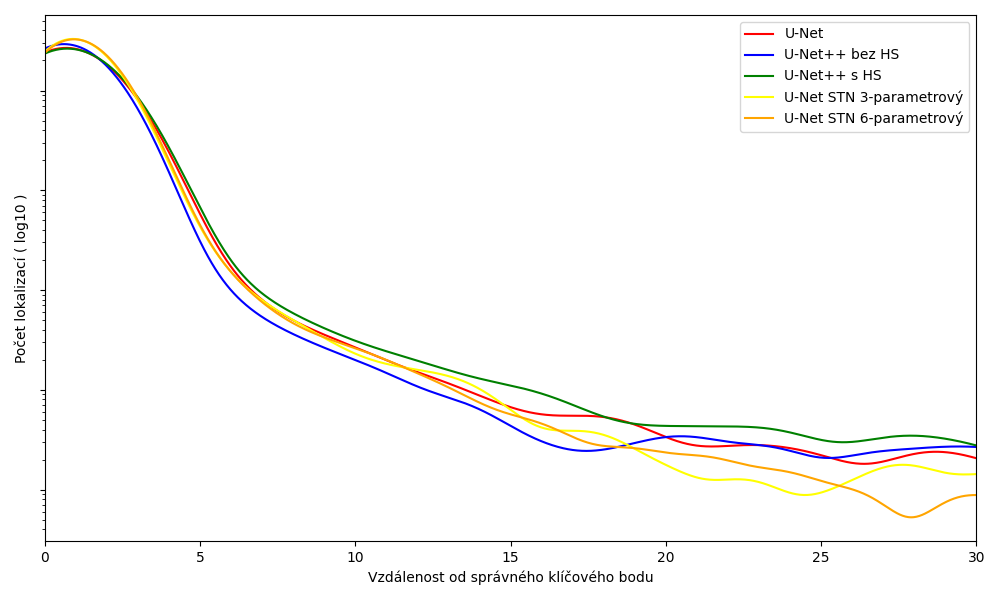
\includegraphics[width=0.8\textwidth,keepaspectratio]{Figures/plots/loc_distance.png}
\caption[Chyba lokalizace modelů]{Chyba lokalizace zobrazená pomocí KDE v logaritmickém měřítku }
\label{fig:loc_distance}
\end{figure}

Obdobně vykazuje podobné rozdíly mezi modely i síla lokalizace (maximální hodnota na výstupním kanále sítě v bodě lokalizace) v následujícím grafu \ref{fig:loc_strength}:

\begin{figure}[H]
\centering
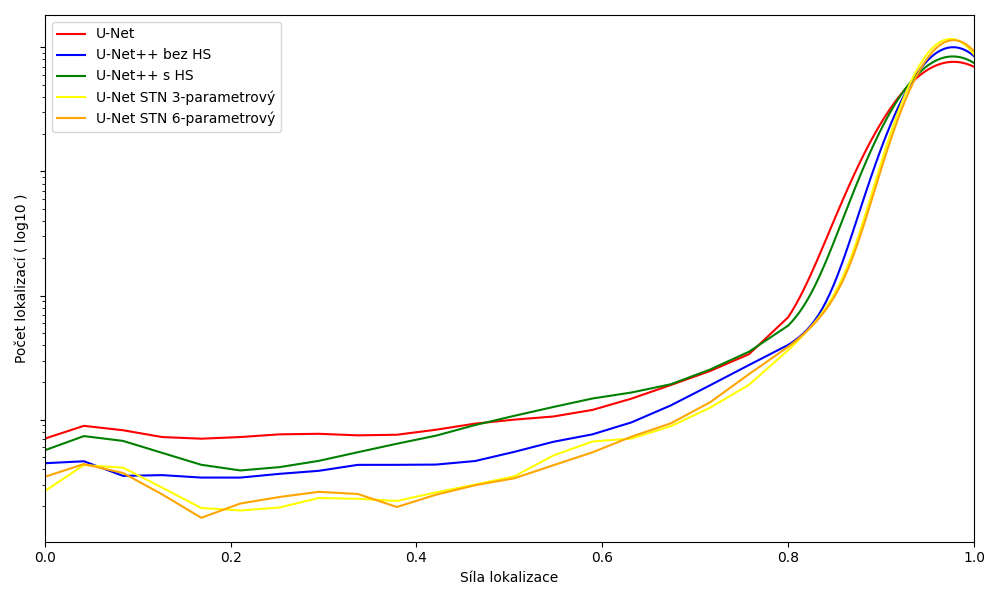
\includegraphics[width=0.8\textwidth,keepaspectratio]{Figures/plots/loc_strength.png}
\caption[Síla lokalizace modelů]{Síla lokalizace zobrazena pomocí KDE v logaritmickém měřítku }
\label{fig:loc_strength}
\end{figure}

Kompletní a obsáhlý přehled výsledků lokalizace také i mezi kanály může být viděn v tabulce \ref{tab:mean_std_channels}:

\begin{table}[ht]
    \centering
    \begin{tabular}{lrrrrr}
    \toprule
    Kanál & U-Net & U-Net++ bez HS & U-Net++ s HS & U-Net STN 3p & U-Net STN 6p \\
    \midrule
0 & \textbf{1,5$\pm$0,81px} & \textbf{0,79$\pm$0,66px} & 1,18$\pm$0,84px & 0,94$\pm$1,07px & 0,84$\pm$1,08px \\
1 & 0,73$\pm$0,78px & 0,74$\pm$0,65px & \textbf{0,74$\pm$0,83px} & 0,69$\pm$1,0px & \textbf{0,68$\pm$1,04px} \\
2 & \textbf{1,84$\pm$0,94px} & \textbf{0,98$\pm$0,84px} & 1,46$\pm$0,99px & 1,0$\pm$1,17px & 1,52$\pm$1,21px \\
3 & 1,85$\pm$1,0px & 1,79$\pm$0,99px & \textbf{2,08$\pm$1,13px} & 1,8$\pm$1,29px & \textbf{1,47$\pm$1,27px} \\
4 & \textbf{0,96$\pm$0,6px} & \textbf{1,21$\pm$0,53px} & 1,02$\pm$0,66px & 1,03$\pm$0,88px & 0,97$\pm$0,93px \\
5 & 0,67$\pm$0,59px & 0,58$\pm$0,46px & 0,69$\pm$0,55px & \textbf{0,7$\pm$0,82px} & \textbf{0,49$\pm$0,8px} \\
6 & 0,95$\pm$0,69px & 1,24$\pm$0,64px & \textbf{1,28$\pm$0,81px} & \textbf{0,62$\pm$0,96px} & 0,68$\pm$1,03px \\
7 & 1,16$\pm$0,83px & 1,13$\pm$0,74px & \textbf{1,35$\pm$0,84px} & 0,77$\pm$1,05px & \textbf{0,7$\pm$1,13px} \\
8 & 0,62$\pm$0,52px & 0,72$\pm$0,55px & \textbf{0,8$\pm$0,49px} & \textbf{0,42$\pm$0,79px} & 0,43$\pm$0,82px \\
9 & 0,97$\pm$0,85px & 1,06$\pm$0,76px & \textbf{1,07$\pm$0,88px} & \textbf{0,89$\pm$1,13px} & 0,9$\pm$1,17px \\
10 & \textbf{2,17$\pm$0,85px} & 2,03$\pm$0,81px & 2,16$\pm$0,99px & \textbf{1,86$\pm$1,12px} & 1,97$\pm$1,16px \\
    \bottomrule
    \end{tabular}
    \caption[Průměr a směrodatná odchylka vzdálenosti mezi kanály a sítěmi]{Průměr a směrodatná odchylka vzdálenosti lokalizace mezi kanály a sítěmi}
    \label{tab:mean_std_channels}
\end{table}


\endinput